\documentclass[11pt]{article}
\usepackage[utf8]{inputenc}
\usepackage[T1]{fontenc}
\usepackage{lmodern}
\usepackage{amsmath,amssymb,mathtools}
\usepackage{booktabs,tabularx,array}
\usepackage{graphicx}
\usepackage[margin=1in]{geometry}
\usepackage{enumitem}
\usepackage[hidelinks]{hyperref}
\usepackage{xcolor}
\setlength{\parindent}{0pt}
\setlength{\parskip}{5pt}
\setlist[itemize]{leftmargin=1.4em,itemsep=2pt,topsep=2pt}
\setlist[enumerate]{leftmargin=1.7em,itemsep=2pt,topsep=2pt}
\renewcommand{\arraystretch}{1.18}
\emergencystretch=3em
\sloppy
\allowdisplaybreaks

\title{Typed ledgers and the limits of compensatory sustainability indicators}
\author{}
\date{}
\begin{document}
\maketitle
\section{Abstract}
\begin{abstract}
Ecological-economic assessment often places heterogeneous material stocks, services and depletion indicators on a common scalar scale. This creates two distinct errors. A surplus in one component can compensate for a deficit in another in the reported aggregate, while a quantity expressed in years can be mistaken for a physical exhaustion horizon. We develop a typed stock--flow ledger that treats substance classes, conversions, boundary flows and service readouts as different declared objects. Conservation follows from the incidence structure, nonnegativity from donor limitation, and barrier safety is certified componentwise rather than inferred from a weighted aggregate. We then distinguish gross turnover intensity, a frozen-rate local ratio and a scenario-conditioned hitting time. Three published records are classified without promoting them to forecasts: a G3P groundwater anomaly-persistence index, a USGS phosphate reserve-life ratio and a fisheries removals-only pressure time. The result is an operational bridge between ecological-economics concerns about weak comparability and a formal accounting discipline: substitution is admitted only through a declared physical conversion or a named economic convention, and an indicator retains the question and boundary that produced it. Formal proofs, extended records, procedures and reproducible computations are delegated to the technical supplement and full-length deposit.
\textbf{Keywords:} ecological economics; strong sustainability; weak sustainability; material-flow accounting; noncompensatory indicators; natural capital; depletion horizons
\section{1. Introduction: two ways an indicator can mislead}
\end{abstract}
Ecological economics has long questioned whether heterogeneous environmental values and critical natural stocks can be safely compressed into one compensatory number (Martinez-Alier et al., 1998; Munda and Nardo, 2009; Neumayer, 2013). The concern is not that every scalar index is useless. A scalar can communicate, rank or trigger further investigation. The concern is that its interpretation can exceed what its construction certifies. If a deficit in an irreplaceable stock is offset by a surplus in another component, the aggregate can look adequate while the conjunctive condition needed for sustainability has failed.
A related error concerns ``time to depletion''. A reserve-life ratio is a division of an economically declared reserve by current production. A groundwater anomaly-persistence statistic extrapolates a fitted trend to a historical minimum of an anomaly product. A fisheries removals-only time divides a biomass margin by current fishing mortality after deliberately omitting recruitment, growth and future management. All three can be measured in years. They are not automatically the same object, and none becomes a forecast merely through its unit.
The paper's central claim is therefore methodological. Sustainability assessment should expose the boundary at which a value judgment, classification convention or physical conversion enters the account. A typed ledger does this by keeping unlike substance classes separate, representing conversions as explicit routed fluxes, and treating ecosystem services as readouts of a physical and institutional state rather than as additional conserved matter. The framework does not settle the worth of a service or the ethics of substitution. It states what a physical accounting claim requires before it can be certified.
This version is tailored to an ecological-economics article. It retains the formal objects needed to make the argument exact, but delegates full proofs and procedural detail to the technical supplement. The full-length deposit contains the extended theorem set, the standards commentary, public-data provenance, reproducible arithmetic and the complete source line.
\subsection{1.1 What this framework does---and does not---claim}
The framework is not a universal welfare index, a replacement for environmental-economic accounts or a calibrated model of any named aquifer, mineral deposit or fishery. It is an accounting and classification layer. Its strongest claims concern the structure of declared ledgers: internal transfers cancel in the incidence operator, donor limitation preserves nonnegative stocks, componentwise barriers cannot generally be replaced by a nonnegative weighted sum, and a time-like quantity retains the boundary and rate assumptions that define it.
The applied records are included because a formal framework becomes useful when it can refuse a common misreading of real public products. Their evidentiary status is intentionally different from that of the theorem set. The G3P result is a statistical classification of an anomaly record. The phosphate result is arithmetic on an economic reserve class. The fisheries result is a gross-removals comparison process. None is presented as a forecast or as an empirically identified completion of the closed ledger.
This separation also protects the ecological-economic argument from a false choice between ``formal'' and ``applied''. Formal conditions identify what a claim would require; public records show where a familiar claim does not meet those conditions. The policy value is the resulting request for a missing stock, boundary, feedback or model---not a new universal index.
\section{2. The typed ledger as an ecological-economic boundary}
Let \(x(t)\in\mathbb{R}_+^n\) denote stocks in physical compartments, \(v(t)\in\mathbb{R}_+^J\) primitive internal fluxes, and \(b(t)\) declared boundary flows. The ledger is
\[\dot x=S_{\mathcal T}v+b.\]
The subscript is substantive. The incidence representation shares a formal language with compartmental and reaction-network models (Jacquez and Simon, 1993; Feinberg, 2019). The type structure \(\mathcal T\) declares substance classes, compartment units, and conversion coefficients. A transfer has signed entries within one class. A conversion joins distinct classes only through its declared coefficient and named process. A number is not summable with another number merely because both are recorded in kilograms, tonnes or monetary units.
A moiety-composition matrix \(C\) produces the conserved readouts \(S=Cx\). An ecosystem service, economic output or institutional response is instead a readout \(O(x,u,\theta)\). This distinction matters for ecological economics because service flows and natural assets can be related without being the same conserved object. A high output can reflect regeneration, stored support or liquidation of a slowly replenishing pool; the ledger must say which.
Three predicates are separated:
\begin{itemize}
\item \textbf{Accounting consistency:} the balance law holds for the declared trajectory.
\item \textbf{Conservation consistency:} each declared conserved covector lies in the left null space of the incidence operator.
\item \textbf{Barrier safety:} the componentwise readout remains between declared lower and upper bounds.
\end{itemize}
Donor limitation supplies the positivity condition: a primitive outflow must vanish when its source compartment is empty. Yield below one must route the missing fraction to a represented compartment or a declared boundary. These are not stylistic preferences. Without them, a balanced table can create phantom mass or export from an empty donor.
\subsection{2.1 Stocks, flows, services and values are not one object}
The ecological-economic boundary becomes especially important when a paper moves between physical and value language. A stock is a state variable with a type and unit. A flow changes a stock or crosses a declared boundary. A service is a feasible output or observation associated with a state and an operation. A monetary value is a valuation relation. The framework permits these objects to be linked, but does not allow one to inherit another's conservation law by analogy.
This distinction also determines the meaning of a conversion. If one type is transformed into another, the coefficient and route must be named. If a technology avoids the use of a material, that is a change in the production or readout relation, not necessarily a conversion in the material ledger. If a substitute is recycled into the original pool, the return flux and its losses must be represented. If it is imported from outside the system, it is a boundary input. The same word---substitution---can therefore refer to physically different operations, and the ledger requires the author to say which one is meant.
A componentwise safety condition is likewise not an ethical ranking of components. It is a declaration that certain lower or upper bounds are jointly required for the object under study. The framework can represent a policy choice about a critical threshold; it cannot derive that choice from incidence algebra. This is the appropriate division between formal accounting and ecological-economic judgment: the former makes the implication checkable, while the latter supplies the boundary and its significance.
The typed account is compatible with a scalar communication index, but the scalar must carry its status. A positive aggregate may be a useful alarm, ranking or summary. It is not a substitute for the vector safety set unless the feasible domain supplies an additional implication from the scalar to every component. The absence of that implication is a mathematical property of the domain, not a preference for one school of ecological economics.
\begin{figure}[htbp]
\centering
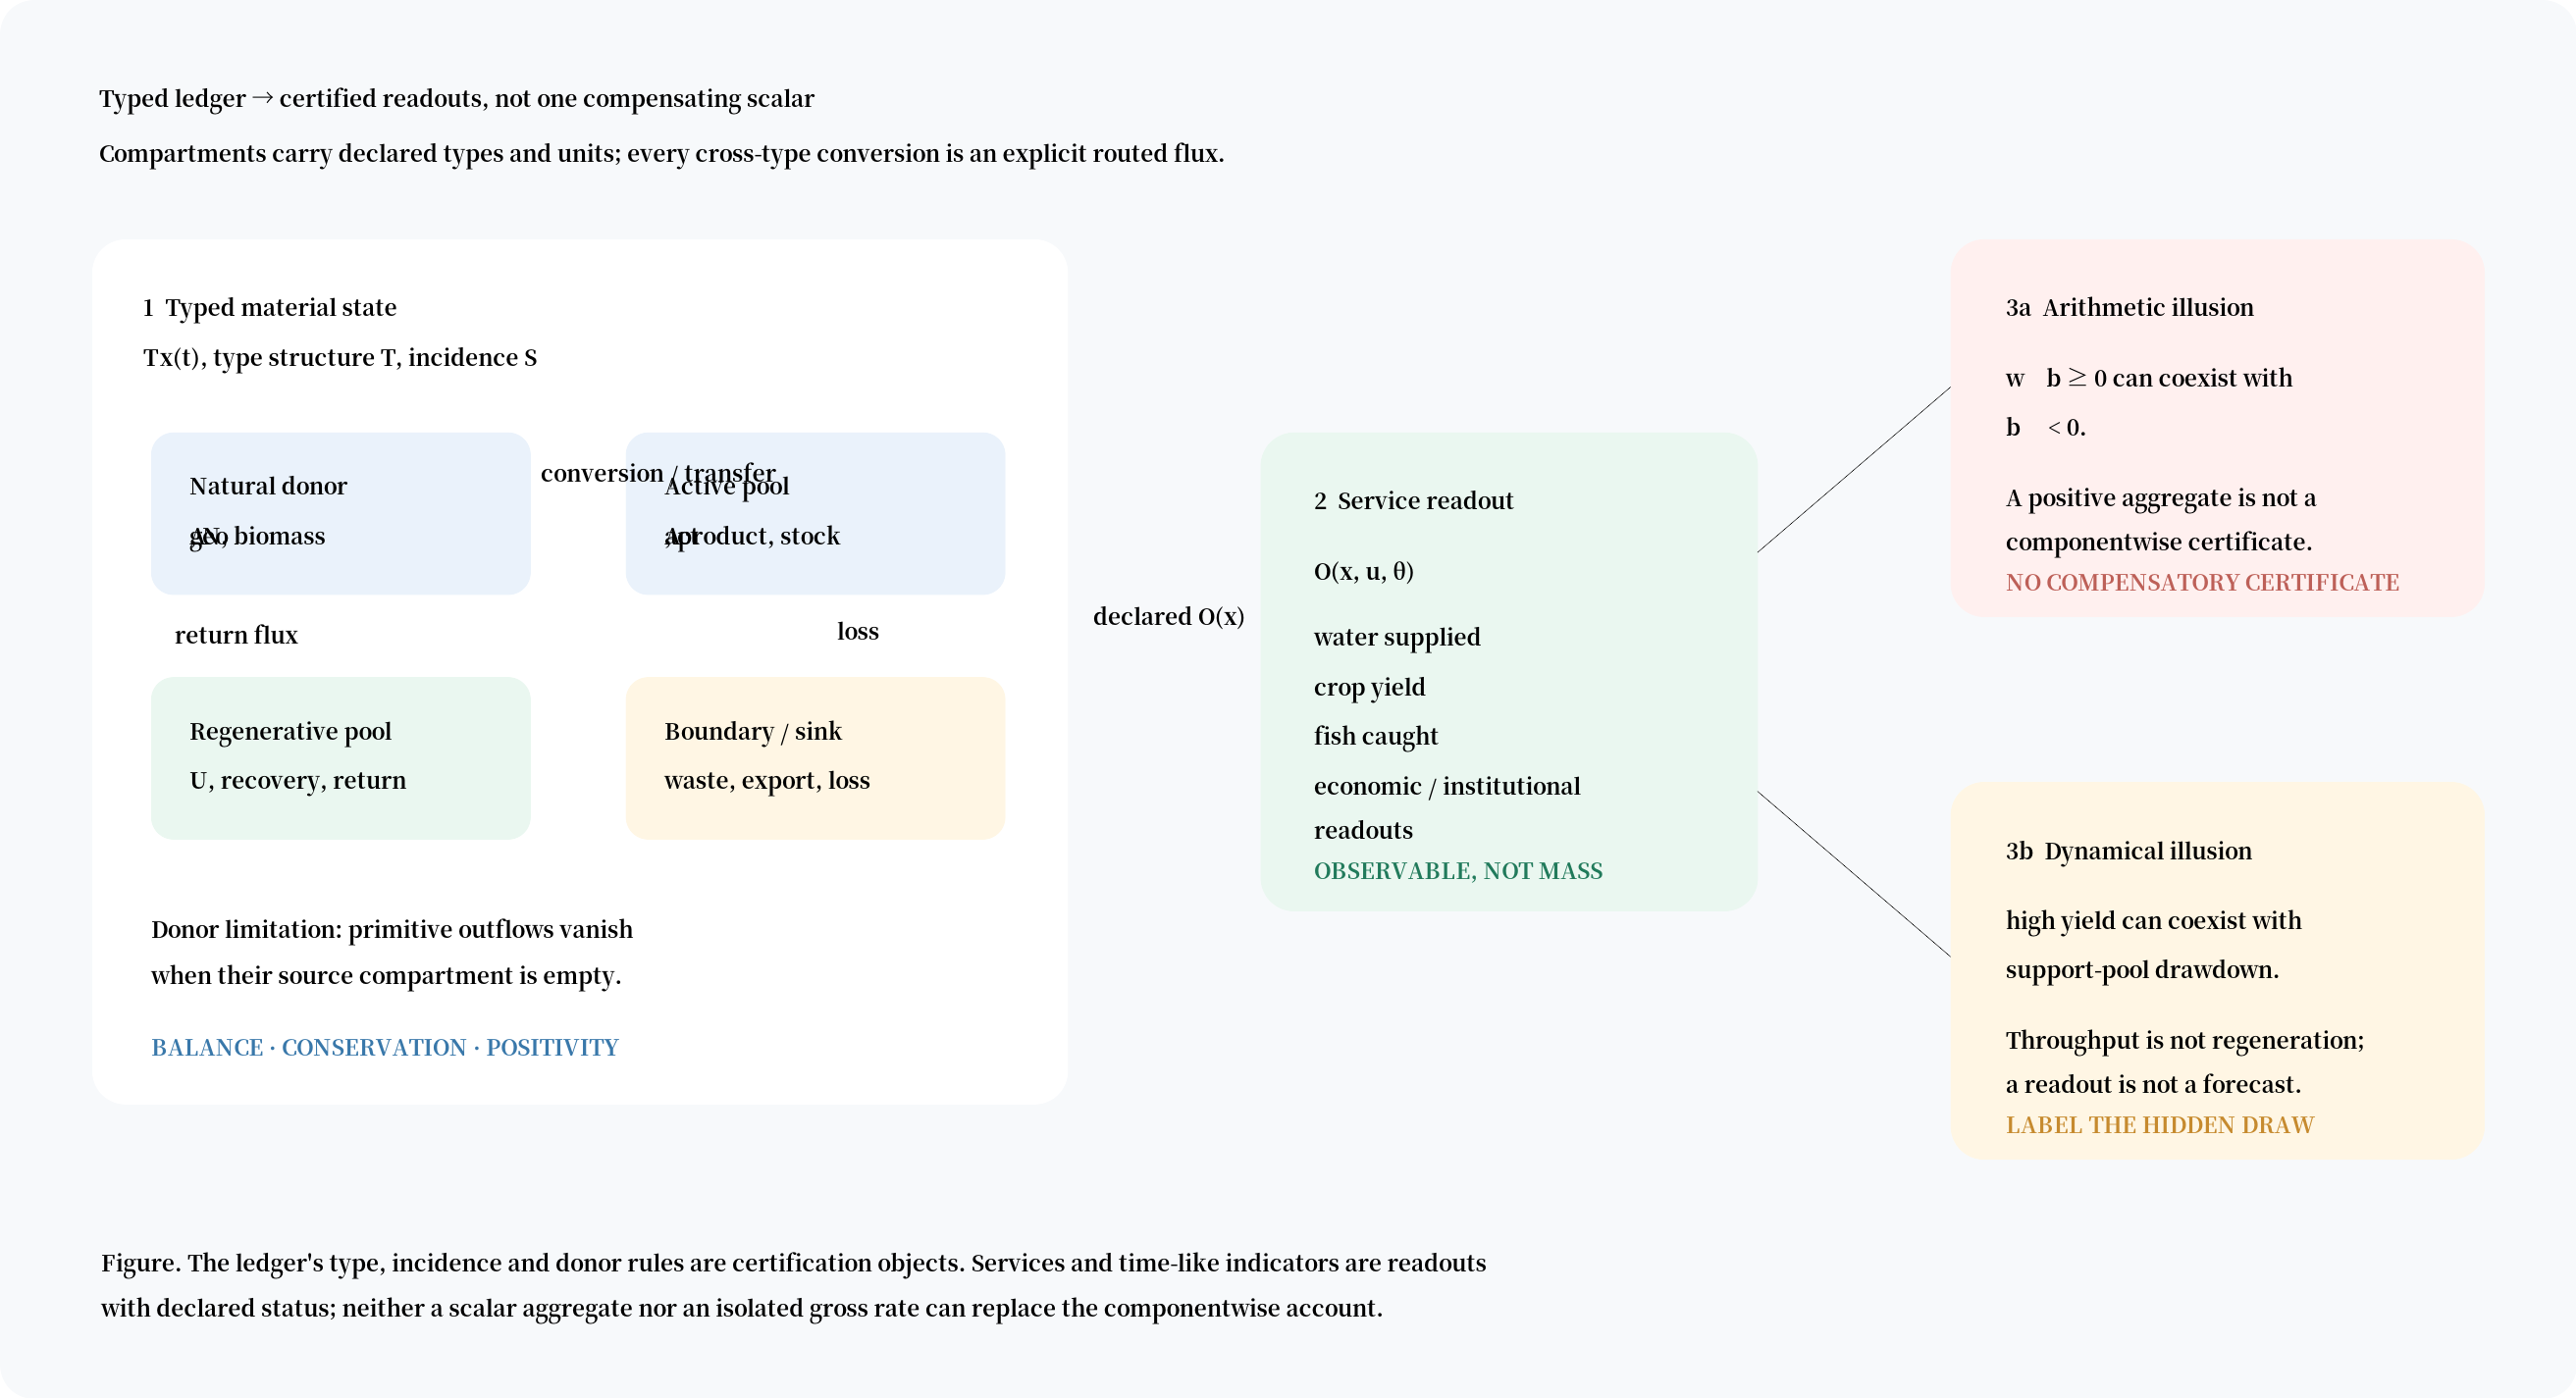
\includegraphics[width=\linewidth]{../assets/typed_ledger_readout.png}
\caption{Typed ledger, readouts and aggregation failures}
\end{figure}
\medskip
\textbf{Figure 1.} A typed account keeps material stocks and service readouts distinct. The two red/amber routes are the arithmetic and dynamical forms of the productivity illusion: a scalar can conceal a deficit, and a high service output can coexist with support-pool drawdown.
\section{3. Noncompensation and the operational meaning of strong sustainability}
The certification state is
\[\mathrm{Cert}=(\mathsf{Typed},\mathsf{Balanced},\mathsf{Conserved},\mathsf{Positive},\mathsf{Admissible},\mathsf{Safe},\mathsf{Adequate\ service},\mathsf{Closed}).\]
Each entry is \texttt{established}, \texttt{not established} or \texttt{not applicable}. This avoids treating an unmeasured parameter as a refutation and avoids turning a descriptive index into a model it does not contain.
The ecological-economic force of the type structure appears in the safety set
\[\mathcal{K}(t)=\{x\ge0:\underline B(t)\le Cx\le\overline B(t)\}.\]
The criterion is conjunctive. All declared critical-component bounds must hold; no weighted aggregate is used as the certificate. Let \(b\) be a feasible balance vector and let \(w\ge0\). Whenever the feasible domain contains \(b_i<0\) with \(w^\top b>0\), the scalar condition is compatible with a critical deficit. This can be constructed for every nonzero nonnegative \(w\) by increasing another component. Thus the result is not an argument against communication indices. It is a limit on what they can certify.
A simple witness uses \(w=(1/2,1/2)\) and \(b=(-2,3)\). The reported aggregate is \(0.5\), but the first component is below zero. The same distinction appears in event times: the two states \((2,98)\) and \((50,50)\) can have the same aggregate trajectory \(Z(t)=100e^{-t}\) while crossing a unit component barrier at \(\log2\) and \(\log50\). An aggregate trajectory cannot transport a component event time.
This is the formal content behind a noncompensatory reading of strong sustainability. The framework does not assert that every strong-sustainability judgment is reducible to one physical inequality. It says something narrower and checkable: cross-type substitution cannot be used as an accounting certificate unless a conversion, coefficient, destination and boundary status have been declared. Within a declared class, a conversion may be physically admissible; across disconnected classes, the ledger supplies no conservation law that prices one class against another.
\subsection{3.1 What the formal results add}
The structural proofs establish four useful separations. First, internal transfers cancel in the natural-block mass identity; only declared extraction and limiting boundary loss change the total. Second, donor limitation makes the nonnegative orthant forward invariant, so positivity is a property of the primitive flux declaration rather than an after-the-fact clipping operation. Third, positive extraction excludes an interior rest point in the closed finite-donor block, while the zero-extraction rest set has distinct extinction, carrying-capacity and frozen-biomass faces. Fourth, extraction is integrable over every finite donor budget. These results do not turn a public indicator into a calibrated dynamic model; they establish what follows once a typed physical ledger has been declared.
The flux-reconstruction identity and conservation reduction are particularly relevant to strong sustainability. A conservation law can show that a total is preserved or changed only through boundary flow, but it does not show that each critical component remains above a moving barrier. Conversely, a trajectory can remain within a declared barrier while its flux decomposition silently violates a conservation or yield-routing rule. The certification layers therefore cannot be collapsed into one ``sustainability score''.
The envelope theorem provides a conservative alternative when exact trajectories are unavailable. Bounds on the declared fluxes integrate to bounds on each moiety readout; if those bounds stay within the componentwise barriers, every compatible trajectory is safe on the declared horizon. The result is only as strong as the flux box, barrier and horizon declarations. It is a certificate under stated uncertainty, not a prediction of an unmodelled world.
The full-length proof record also establishes a non-reduction boundary between the closed physical ledger and open institutional delay models. They may share an exact decline-pressure identity, but an imposed recharge, omitted turnover or institutional control remains a different boundary object. This prevents an ecological-economic model from importing the equilibrium or periodic results of one completion into another merely because the notation looks similar.
The weak/strong distinction can therefore be read as an operational regime interpretation, alongside the ecological-economics literature on throughput, critical natural capital and the limits of the two paradigms (Daly, 1990; Ekins et al., 2003; Neumayer, 2013). In a weak regime, the declared material cycle and substitution routes close at the relevant throughput and time scale. In a strong regime, closure fails or a critical component/barrier binds, so a scalar compensation is not an available certificate. This is not promoted to a theorem here because a theorem would require a complete definition of closure maps, admissible substitutions, boundary flows and time horizon. The statement is an interpretation of the declared ledger objects, not a universal empirical law.
\section{4. Three depletion quantities that should not share one name}
For an active pool \(A\) above a declared threshold \(A_{\min}\), define gross turnover and support coverage by
\[J_A^{\mathrm{gross}}=g(X,A)/A,\qquad H_A^{\mathrm{gross}}=(A-A_{\min})/g(X,A).\]
These answer a dependency or throughput question. The frozen local ratio is
\[H_A^{\mathrm{loc}}(t)=\frac{A(t)-A_{\min}}{[-\dot A(t)]_+},\]
with \(+\infty\) when the current net derivative is nonnegative. A scenario-conditioned hitting time is
\[T_A(x_0;\pi,d)=\inf\{t\ge0:A^{\pi,d}(t;x_0)\le A_{\min}\}.\]
It requires a model, policy, disturbance history and barrier. A uniform drift bracket can bound the relationship between the local ratio and the hitting time; absent that assumption, the local ratio is a frozen-rate diagnostic.
\begin{tabularx}{\linewidth}{XXXXX}
\toprule
Record & Data boundary & Quantity & Ecological-economic reading & Not licensed by the construction \\\\
\midrule
G3P groundwater & anomaly product and reference window & four-basin persistence values about 2.7, 7.9, 9.5 and 21.4 years & record-relative statistical stress under a trend convention & aquifer exhaustion or a physical stock forecast \\\\
USGS phosphate & economic reserve class and production & approximately 309-year reserve-life ratio & arithmetic horizon of a changing economic classification & geological exhaustion or fixed donor depletion \\\\
Fisheries & SSB, reference biomass and current \(F\) & selected-cohort median about 1.8 years; broad public cohort 3.39 years & gross removals pressure under an incomplete comparison process & demographic hitting time or closure date \\\\
\bottomrule
\end{tabularx}
\medskip
The groundwater index is relative to the product's own anomaly record. A physical local ratio requires an absolute stock estimate and net stock derivative. The phosphate ratio is approximately \(74{,}000{,}000/240{,}000=309\) years on the pinned U.S. Geological Survey record (U.S. Geological Survey, 2026), in the setting discussed by Illakwahhi et al. (2024); a resource-threshold calculation of approximately 1,125 years answers a different question. The difference is not a contradiction: reserves are an economic classification whose membership changes with prices, technology, exploration and regulation.
The fisheries quantity is
\[\Theta_F=\frac{\log(\mathrm{SSB}_{\mathrm{now}}/B_{\lim})}{F_{\mathrm{now}}},\]
which is the crossing time of the comparison process \(\dot B=-F_{\mathrm{now}}B\). Recruitment, somatic growth, maturation, natural mortality, density dependence, environmental forcing and future management are omitted. The selected 43-stock cohort includes zero entries for stocks at or below the reference; the positive sub-cohort and the broad public-release comparison show why the vintage and cohort are part of the number. A short number is not evidence of a short biological horizon.
The three records produce three different next questions. Groundwater requires absolute storage and recharge evidence. Phosphate requires the reserve/resource boundary, reclassification and recycling assumptions. Fisheries requires a demographic model if the policy question concerns population viability. An indicator is more useful when it identifies the next missing object than when it borrows the authority of a forecast.
\subsection{4.1 Status-labelled applications rather than synthetic comparability}
The comparison table is not a ranking of basins, reserves and fisheries. It is a table of construction types. The G3P values come from G3P v1.12 (G\``untner et al., 2024) and depend on the product window, basin mask, anomaly reference and fitted trend. The phosphate value depends on which reserve classification and production vintage are placed in the quotient. The fisheries values use the RAM Legacy record (Ricard et al., 2012) and depend on cohort selection, reference convention, zero entries and database release. These dependencies are part of each number's meaning.
The same discipline applies to the inverse-horizon illustration in the full-length article. A positive aggregate made from four basin indices and a phosphate ratio is retained as a non-example: it demonstrates that unlike records can be made to look comparable when their types and boundaries are not. The framework does not treat the positive aggregate as a sustainability score. It uses it to show why a scalar can be communicatively convenient and physically uninformative.
A status-labelled application therefore reports at least four fields: the object measured, the operation used, the source and vintage, and the strongest permissible interpretation. This is a more demanding standard than attaching a caveat after a headline number, because the status travels with the quantity into tables, figures and policy summaries. It also makes disagreement productive: two analysts can locate whether they differ over the source, operation, boundary or interpretation.
\section{5. Productivity, natural capital and policy salience}
The framework separates two senses of the productivity illusion. The arithmetic sense is a surplus in one balance component compensating for a deficit in another. The dynamical sense is a maintained service or yield supported by drawdown of groundwater, soil carbon, bioavailable nutrients or a parent mineral pool. In both cases the system can look productive while the object that makes the output possible is being depleted.
This distinction gives the framework a policy use without making a policy forecast. A positive aggregate should trigger a componentwise check, not a declaration of adequacy. A reserve-life ratio should trigger inspection of the classification and reclassification rules, not a geological countdown. A removals-only fisheries time should trigger a request for an explicit population model, not a closure date. A groundwater anomaly should trigger an absolute-storage identification plan, not a claim that a basin will fail in the reported number of years.
The typed ledger also clarifies what ``substitution'' means. A recycled flux returning to a regenerating pool is a routed material operation. A new technology that avoids one material is a change in the production/readout relation. A monetary willingness to substitute is a valuation statement. These can interact, but they are not interchangeable entries in a conservation equation. Strong sustainability becomes operational precisely at the point where a declared critical stock cannot be certified through a cross-type scalar surplus.
The relation to environmental-economic accounts is deliberately limited. The standards and MFA literature provide stock, flow, asset, residual and service-accounting conventions (Eurostat, 2001; Fischer-Kowalski et al., 2011); the present framework adds an operator-level audit of types, conversions, donor limitation and componentwise barriers. Companion B carries the extended standards comparison. This article does not claim that an accounting standard supplies a depletion horizon, nor that a typed ledger replaces the standard's measurement boundary.
\subsection{5.1 From indicator criticism to a usable policy question}
The framework's policy salience comes from changing the question asked of an indicator. Instead of asking ``what is the depletion date?'', the analyst asks four narrower questions:
\begin{enumerate}
\item What physical or economic object is in the numerator?
\item What rate, trend or model is in the denominator or drift term?
\item Which threshold is being crossed, and who declared it?
\item Which missing stock, boundary flow or feedback would change the interpretation?
\end{enumerate}
For the groundwater record, the answer identifies the need for absolute storage and recharge information. For phosphate, it identifies the reserve/resource boundary and the assumptions governing reclassification and recycling. For fisheries, it identifies the need for a demographic or management model. These are not policy forecasts. They are measurement and modelling requirements that prevent a descriptive statistic from being used as a decision object it cannot support.
This also clarifies the relationship between weak and strong sustainability. A weak-sustainability reading may permit a service to be maintained by a substitution or return route, but the route must be declared and its losses assigned. A strong-sustainability constraint becomes binding when a critical component cannot be replaced within the declared type structure or when closure capacity falls below the required throughput. The account therefore does not infer strong sustainability from a moral label; it locates the physical or boundary condition at which compensation ceases to be a valid certificate.
\subsection{5.2 A compact reader-facing crosswalk}
\begin{tabularx}{\linewidth}{XXX}
\toprule
Assessment question & If the record is adequate & If it is not adequate \\\\
\midrule
Are unlike material classes being added? & A declared conversion or common type makes the sum interpretable. & Keep components separate; do not repair the gap with weights. \\\\
Is a service maintained by regeneration? & The supporting pool and return flux are represented and bounded. & Label the service as a readout and identify the unobserved support draw. \\\\
Is a time-like number a horizon? & A stock, barrier, model/scenario and drift class are declared. & Report a ratio, index or pressure time with its exact status. \\\\
Does a cycle close? & Return capacity covers the declared use over the stated horizon. & Report the deficient cut or boundary input rather than calling the system circular. \\\\
\bottomrule
\end{tabularx}
\medskip
The crosswalk is intentionally operational. It gives an analyst a route from an indicator critique to a record request without turning the framework into a universal ranking index.
\subsection{5.3 Relation to weak comparability and natural-capital arguments}
The framework's algebraic obstruction is narrower than the ecological-economics literature's full critique of commensuration. It does not claim that all values are incommensurable, nor that no composite index can be useful. It shows that a nonnegative linear aggregate over mixed-sign component balances is not, without additional domain restrictions, a certificate that every component is adequate. This gives the weak-comparability concern a checkable accounting location.
The relation to strong sustainability is similarly conditional. Critical natural capital is not represented by declaring one weight ``large enough''; it is represented by a component and a barrier whose failure cannot be certified away by another component's surplus. A substitution route can be considered only after its physical or institutional mechanism is declared. A return route can support a weak-sustainability reading only if it closes at the relevant throughput and horizon. If the return capacity, donor stock or barrier condition fails, the strong constraint is not a rhetorical preference but a binding object of the account.
This formulation leaves room for values, institutions and policy choice. The author or institution may choose the barrier, service requirement or reporting boundary. The formal ledger then records the consequences of that choice and prevents a later scalar summary from erasing them. The result is an interface between ecological-economic judgment and physical accounting, not a claim that algebra can choose the judgment.
\section{6. Certification as a usable method}
The method is designed to be read as a sequence rather than as a single score. The user declares compartments, units, types, conversions, fluxes, boundaries, barriers, a horizon and the source vintage. The incidence operator is checked first. Balance and conservation are then checked independently. Positivity and barrier safety are checked only on the trajectory or scenario for which their inputs exist. Closure and service adequacy are reported only when their demand and return objects are declared.
Companion A provides the full practitioner route: a compartment table, flux table, incidence operator and boundary schedule; eight predicate procedures; three linear programmes; status semantics; vintage rules; and the reproduction bundle. The full-length deposit contains the extended proofs and the executable arithmetic behind the aggregation witness, persistence simulation, curvature correction and reserve-life comparison. The current code is a reproduction exhibit, not a supported software package; a software-journal route would require an API, tests, examples, benchmarks and installation documentation.
\subsection{6.1 Evidence levels and reproducibility}
The paper keeps four evidence levels separate. Algebraic identities and theorem proofs are established within the declared ledger. Descriptive arithmetic is established for the pinned public-data record and its protocol. A parameter or barrier that the record does not identify is reported as not established. A predicate that has no live object in a public indicator is not applicable. This vocabulary prevents a clean arithmetic calculation from borrowing the authority of a dynamic model.
The reproduction bundle mirrors the distinction. One group of scripts runs on declared figures and reproduces the aggregation, curvature and persistence exhibits without a network. A separate analysis record handles the overshoot-date arithmetic and retains retrieval commands, checksums and licence notes. The code does not ingest the quarantined G3P basin rows or claim a supported software product. This separation is deliberately conservative: a reader can reproduce the arithmetic claim without being told that it validates a physical model the data never identified.
For a policy-facing use, the output should therefore be accompanied by a small record: source release, retrieval date, boundary and type declarations, formula, threshold, status and the strongest claim permitted. The full-length deposit supplies the detailed version of this record; the journal article supplies the decision logic.
\section{7. Limitations and conclusion}
The article makes no claim that the groundwater two-pool template is empirically identified, that the phosphate calculation is a geological-reserve model, or that the fisheries calculation is a stage-structured model. Its first-passage processes are declared stochastic surrogates and do not conserve the physical ledger. The weak/strong interpretation is scoped to the declared closure and conversion objects. These limitations are evidence-status information, not after-the-fact disclaimers.
A sustainability assessment can use a scalar for communication and still refuse to use it as a certificate. It can report a number in years and still refuse to call it an exhaustion date. The typed ledger supplies the missing discipline: each physical stock, conversion, service and boundary is named; the certification layer says what follows; and the indicator retains the question and convention that produced it. In that sense, the framework makes strong sustainability operational not by solving every valuation dispute, but by preventing a compensating scalar from masquerading as a componentwise physical result.
\subsection{Data and code availability}
The full-length article, proofs, supplementary records, companions, source-vintage material and executable reproduction exhibits are prepared as a Figshare-ready deposit. The journal version is a target-specific compression of that record.
\section{References}
Daly, H.E., 1990. Toward some operational principles of sustainable development. \emph{Ecological Economics} 2, 1--6.
Ekins, P., Simon, S., Deutsch, L., Folke, C., De Groot, R., 2003. A framework for the practical application of the concepts of critical natural capital and strong sustainability. \emph{Ecological Economics} 44, 165--185.
Eurostat, 2001. \emph{Economy-wide Material Flow Accounts and Derived Indicators: A Methodological Guide}. Eurostat.
Feinberg, M., 2019. \emph{Foundations of Chemical Reaction Network Theory}. Springer.
Fischer-Kowalski, M., Krausmann, F., Giljum, S., et al., 2011. Methodology and indicators of economy-wide material flow accounting: state of the art and reliability across sources. \emph{Journal of Industrial Ecology} 15, 855--876.
G\``untner, A., Sharifi, E., Haas, J., et al., 2024. Global Gravity-based Groundwater Product (G3P), v1.12. GFZ Data Services. https://doi.org/10.5880/G3P.2024.001
Illakwahhi, D.T., Vegi, M.R., Srivastava, B.B.L., 2024. Phosphorus' future insecurity, the horror of depletion, and sustainability measures. \emph{International Journal of Environmental Science and Technology} 21, 9265--9280. https://doi.org/10.1007/s13762-024-05664-y
Martinez-Alier, J., Munda, G., O'Neill, J., 1998. Weak comparability of values as a foundation for ecological economics. \emph{Ecological Economics} 26, 277--286.
Munda, G., Nardo, M., 2009. Noncompensatory/nonlinear composite indicators for ranking countries: a defensible setting. \emph{Applied Economics} 41, 1513--1523.
Neumayer, E., 2013. \emph{Weak versus Strong Sustainability: Exploring the Limits of Two Opposing Paradigms}, 4th ed. Edward Elgar.
U.S. Geological Survey, 2026. \emph{Mineral Commodity Summaries 2026: Phosphate Rock}. USGS.
Ricard, D., Minto, C., Jensen, O.P., Baum, J.K., 2012. Examining the knowledge base and status of commercially exploited marine species with the RAM Legacy Stock Assessment Database. \emph{Fish and Fisheries} 13, 380--398.
\end{document}
